\chapter{Результаты работы конвейера моделей} \label{ch3}

В данной главе рассматриваются результаты работы конвейера моделей и сборщика графа молекул в совокупности. В параграфе \ref{ch3:sec1} приведено качество работы сборщика молекул. В параграфе \ref{ch3:sec2} приведены следующие метрики: среднее расстояние Левенштейна и процент точных совпадений InChI-идентификаторов. В параграфе \ref{ch3:sec3} показаны характерные примеры, на которых конвейер ошибается, и предложены меры по исправлению некорректных распознаваний. В параграфе \ref{ch3:sec4} приведены замеры производительности построенного продукта.

\section{Качество сборщика молекул} \label{ch3:sec1}

Сборщик молекул тестировался следующим образом. Из InChI-идентификатора генерировался идеальный вывод конвейера нейросетей. 
Это делалось с помощью функциональности RDKit, позволяющей генерировать векторные изображения молекул. Таким образом, удалось установить точные границы ожидаемых баундбоксов и растеризовать их вместе с самими связями и метками атомов.

Далее полученные данные были переданы на вход сборщика. На выходе был получен InChI-идентификатор, который, в соответствии с ожиданиями, должен точно совпадать со входным идентификатором.

В результате оказалось, что генератор позволяет получить только 92.8\% точных совпадений. При анализе проблемы было выяснено, что 0.8\% несовпадений вызвано некачественной генерацией изображений, когда изображения связей и меток накладываются друг на друга, а остальные 6.4\% вызваны неоднозначностью изображения связи и её метаданных либо неоднозначным соответствием между изображением химической молекулы и её физической структурой.

Ярким примером последней ситуации являются изображения алленов. Это соединения, представляющие из себя углеводороды и их замещённые производные с двумя двойными связями у одного атома углерода общей формулы \textbf{RR'C=C=CR''R'''} \cite{allenes}. Известно, что у таких соединений плоскости, в которых находятся атомы \textbf{R, R', C} и \textbf{C, R'', R'''} соответственно, являются ортогональными. Для того, чтобы отразить эту ортогональность на рисунке, необходимо нарисовать две клиновидных связи. Однако из определения алленов понятно, что молекула, состоящая из двух двойных соединяющих атомы углеродов связей, из концов которых выходят ещё по две одинарные связи, обязательно будет являться именно алленом, а не каким-то другим соединением. Поэтому достаточно указывать только один клин -- для того, чтобы определить, какой из атомов -- R или R'  -- находится ближе к наблюдателю, а какой дальше. Таким образом одну и ту же молекулу можно изобразить как минимум тремя способами \footnote{На самом деле таких способов шесть. Можно указывать клиновидность связей, находящихся в левой части изображения -- \textbf{CR} и \textbf{CR'}}.

\begin{figure}[h!] 
	\center
	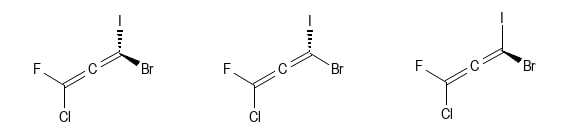
\includegraphics [scale=1.0] {my_folder/images/allene}
	\caption{Три разных изображения одного и того же аллена}
	\label{fig:allenes}
\end{figure}
	
\section{Качество конвейера моделей} \label{ch3:sec2}
Для проведения качественного тестирования моделей были использованы данные, ранее не задействованные при обучении. Было взято 20000 разнообразных молекул и посчитано среднее расстояние Левенштейна. Оно составило 4.32 редакционных изменения.

Процент точных совпадений молекул составил 81.8\%. Учитывая, что точность генератора составляет 92.8\%, можно сделать вывод, что истинная точность конвейера моделей составляет около 88.1\%, что является отличным показателем для object detection задачи, поскольку задача распознавания при таком подходе состоит из большого числа распознаваний, в каждом из которых есть шанс ошибиться и, таким образом, предоставить неточное предсказание для всей молекулы в совокупности.

\section{Типовые ошибки конвейера. Методы устранения} \label{ch3:sec3}

Наиболее часто встречающиеся ошибки связаны с распознаванием меток атомов кислорода и азота с указанием атомов водорода -- $O, NH, NH_2$. Причина заключается в том, что обучающая выборка является несбалансированной: количество меток атомов в несколько раз меньше, чем количество меток связей. Для решения данной проблемы необходимо генерировать набор данных, содержащий большее количество меток атомов при том же количестве связей. Реализация данной функциональности предполагает разработку алгоритма, который сможет менять атомы углерода на другие атомы, соблюдая при этом требования, касающиеся валентности: количество связей, которые исходят из данного атома, должно быть в списке возможных валентностей. Такой алгоритм может быть реализован при дальнейших исследованиях в рамках данной работы.

\begin{figure}[h!] 
	\center
	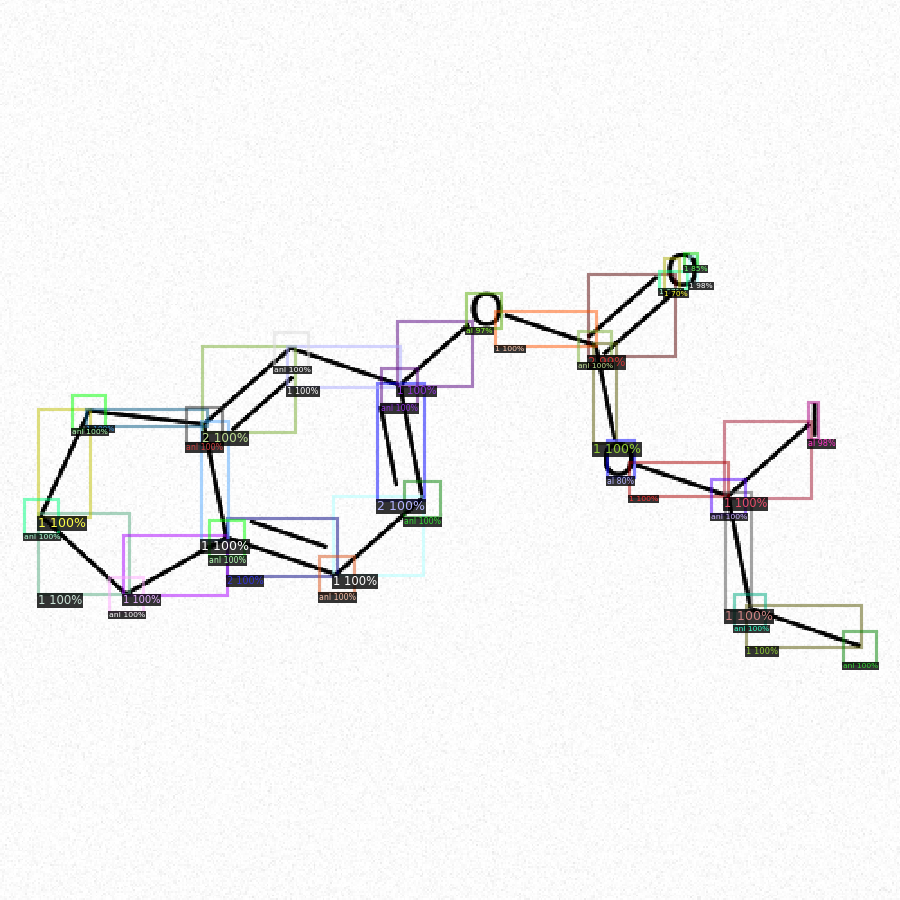
\includegraphics [scale=0.25] {my_folder/images/inference1}
	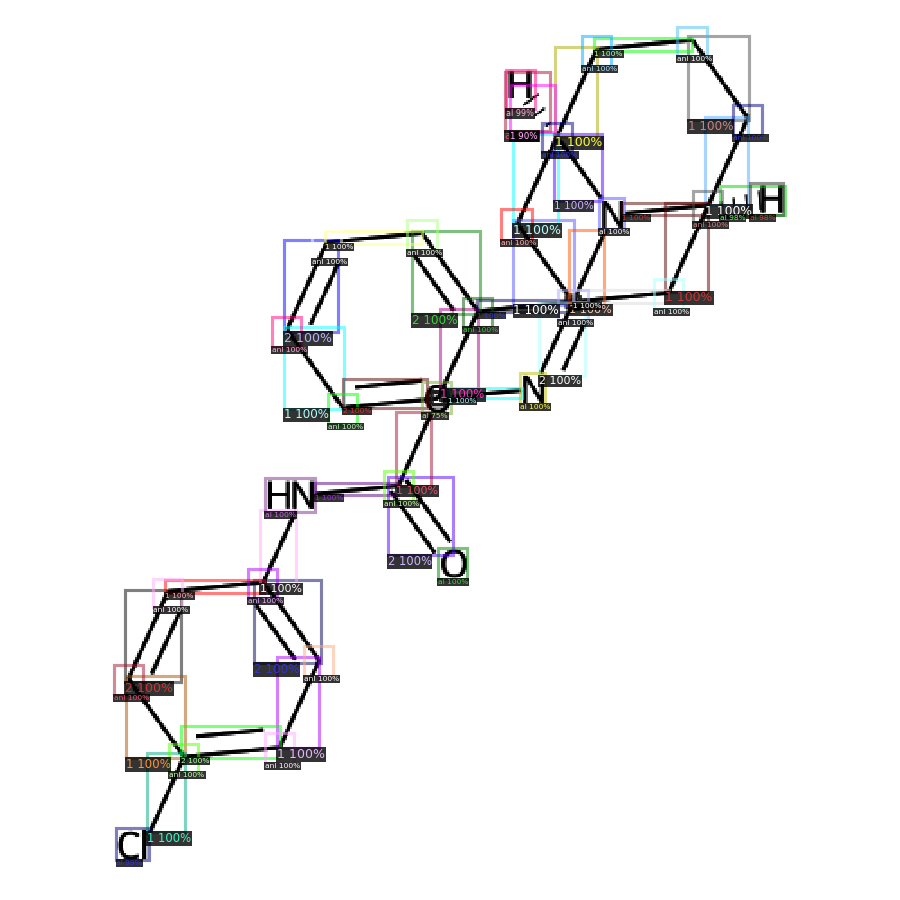
\includegraphics [scale=0.25] {my_folder/images/inference2}
	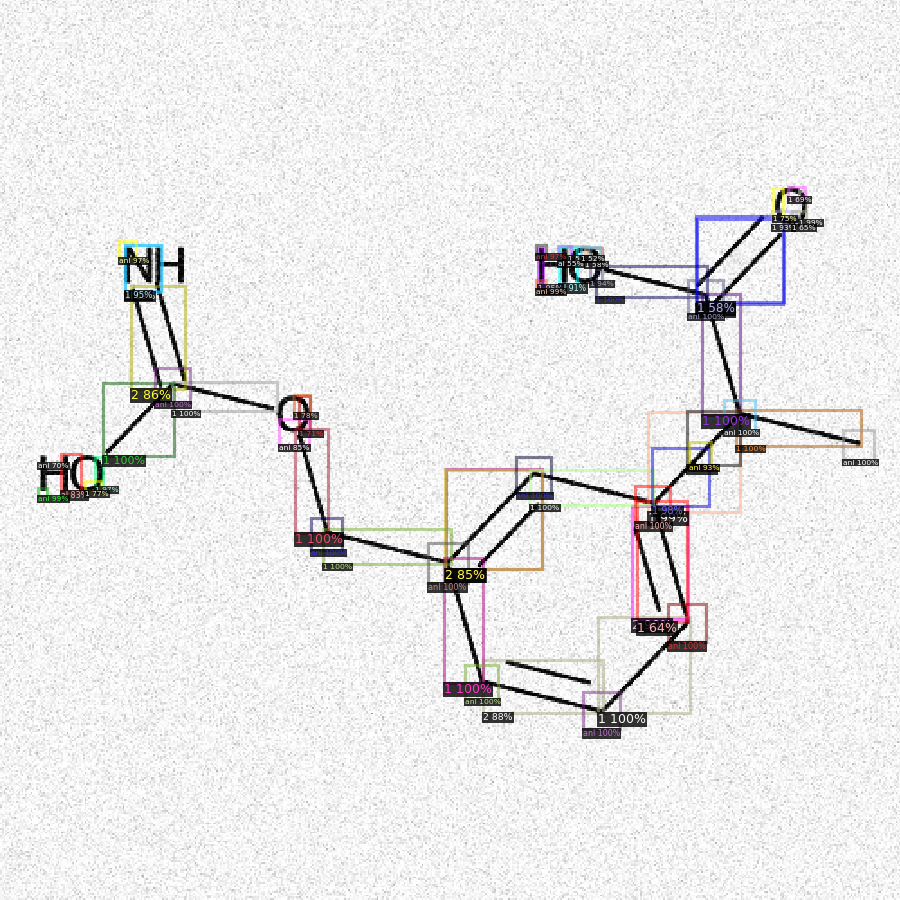
\includegraphics [scale=0.28] {my_folder/images/inference3}
	\caption{Типовые ошибки распознавания Faster R-CNN: некорректно построенные баундбоксы атомов (1) кислорода, (2) водорода, (3) азота}
	\label{fig:mistake}
\end{figure}

Подобные ошибки происходят приблизительно в одном из 15-20 случаев.

\section{Производительность решения} \label{ch3:sec4}

Были произведены замеры производительности на ноутбуке следующей конфигурации:

\begin{itemize}
	\item CPU: AMD Ryzen 5 5600H
	\item GPU: Nvidia GeForce RTX3050
	\item RAM: 16 Gb
\end{itemize}

Для данной конфигурации была производительность решения составила 3.11 изображений в секунду. Из них 45\% уходит на операции RDKit по добавлению элементов во внутреннее представление молекулы и её валидацию. Также около 8\% уходит на обмен данными между CPU и GPU, а оставшиеся 47\% занимает инференс моделей и сборка графа молекулы.


%\FloatBarrier % заставить рисунки и другие подвижные (float) элементы остановиться


%% Вспомогательные команды - Additional commands
%
%\newpage % принудительное начало с новой страницы, использовать только в конце раздела
%\clearpage % осуществляется пакетом <<placeins>> в пределах секций
%\newpage\leavevmode\thispagestyle{empty}\newpage % 100 % начало новой страницы